\chapter{System Description} 

%Pg 66

\section{Configuration}
%Levitating one magnet - repulsive
%	Vs other configurations
%	

For this project, the magnetic levitation system is considered as a SISO (single input, single output) system.  As such, only the bottom coil and magnet are considered as shown in the simplified diagram below.

%INSERT DIAGRAM
\begin{figure}[h]
    \centering
    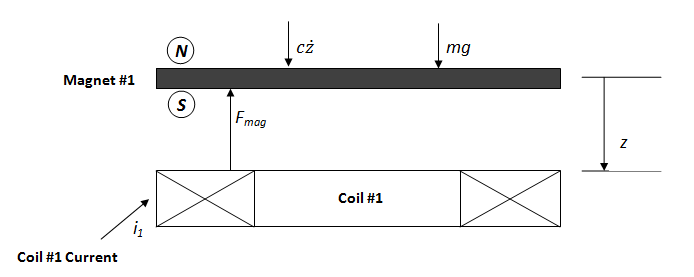
\includegraphics[width=.9\textwidth]{projSys}
    \caption{System Diagram}
    \label{fig:projSys}
\end{figure}

In this model, there are 3 forces acting on the magnet: the force of gravity (mg), the force of friction ($c\dot{z}$) and the force due to the magnetic force form the drive coil ($F_{mag}$).

For the system modeling done in this report, y denotes the output variable, u denotes the input variable and the vector \textbf{x} denotes the state variables.

\section{Inputs, Outputs and State Variables}

\textbf{Input:} The input to the system is the current going into Coil \#1, denoted in the diagram by $i_{1}$.
In terms of system equations we have:
\begin{equation}
u = i_{1}
\end{equation}

\textbf{State variables:} For system model, the state variables are chosen as follows
\begin{itemize}
\item x$_1$:  Disk position
\item x$_2$:  Disk velocity
\end{itemize}
In terms of system equations we have:
\begin{equation}
x = 
\left[
\begin{array}{c}
z\\
\dot{x_{1}}\\
\end{array}
\right]
\end{equation}

\textbf{Output:} The output of the system is the position of the disk magnet, denoted in the diagram by z.
In terms of system equations we have:
\begin{equation}
y = x_{1}
\end{equation}